\chapter{Introdução}

O termo "Internet das Coisas" \space vem sendo usado extensivamente nos últimos anos e isso se deve ao fato, em conjunto com outros como "inteligência artificial", "\textit{Big Data}" \space e "computação em nuvem", de ser protagonista de uma latente revolução industrial, da informação e até da tecnologia de forma geral. A possibilidade de ter dispositivos conectados à internet que podem ser controlados remotamente que podem colher dados que são processados, analisados e usados para tornar processos cada vez mais eficientes e lucrativos tem movimentado um grande mercado em todo o mundo e promete continuar sua expansão. 

Existem certos padrões de comportamento do público consumidor e da indústria diante de  tecnologias emergentes que são caracterizados por descoberta e discussão inicial, difusão entre adotadores precoces e por fim, uso extensivo. Pesquisas indicam que as barreiras iniciais à adoção da "Internet das Coisas" \space vêm sendo quebradas e a nova tecnologia está sendo encontrada não apenas em novas empresas (\textit{startups}) mas também têm atraído atenção da indústria de grande porte \cite{forbes}. 
%referencia da forbes 
%www.forbes.com/sites/louiscolumbus/2018/08/16/iot-market-predicted-to-double-by-2021-reaching-520b/

Outra forte tendência é o uso de diodos emissores de luz (LED) com a finalidade de iluminação tanto para ambientes abertos quanto para ambientes fechados, que já eram usados indicar funcionamento em produtos eletroeletrônicos e equipamentos sinalizadores como lâmpadas de emergência e semáforos. Há alguns anos a tecnologia já era estudada como solução para iluminação mas devido a seu custo elevado, a sua adoção era inviável. O custo dos LEDs vem caindo graças à produção em larga escala e a melhorias na sua eficiência, dessa forma sua viabilidade, em comparação com lâmpadas fluorescentes e incandescentes, vêm aumentando já que o LED apresenta alta eficiência luminosa e longa vida útil apesar de ainda ser mais caro que as tecnologias concorrentes.

A lei de Haitz \cite{haitz}, um análogo da lei de Moore que modela o crescimento da quantidade de transistores em chips ao longo do tempo, declara que a cada década o custo por lúmen(unidade de intensidade luminosa) deve cair por um fator de 10 e a quantidade de luz por gerada por um LED deve aumentar por um fator de 20. Além das previsões sobre custo e quantidade de luz, Roland Haitz também disse que a eficiência luminosa dos LEDs deveria atingir a marca de 200 $lm/W$ (lúmen por watt) e isso resultaria na redução de toda energia gasta com iluminação no mundo (20\% de toda energia elétrica gasta) em 50\%, se todas as fontes fossem LEDs com essa eficiência. Já em 2014 a Cree Inc., uma companhia americana, declarou ter quebrado a barreira dos 300 $lm/W$ \cite{cree} em seus laboratórios após terem atingido importantes marcas de eficiência no passado.

\begin{figure}[ht]
    \begin{center}
    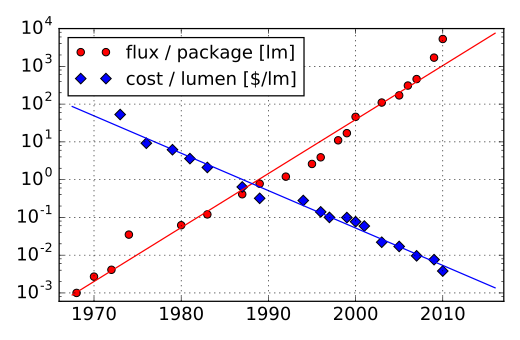
\includegraphics[width=0.5\textwidth]{figuras/haitz.png}
    \end{center}
    \caption[Ilustração da lei de Haitz.]{Ilustração da lei de Haitz com quantidade de luz por LED em vermelho e custo por lúmen em azul.}
    \label{haitz}
\end{figure}

A eficiência elevada e longa vida útil são fatores que vêm impulsionando investimentos nessa área. Uma linha de crédito, com duração de 5 anos, foi aprovada pelo BNDES \cite{bndes2} para fontes luminosas de alta potência em vista da rentabilidade segura que reside na substituição de fontes luminosas convencionais por aquelas que usam LEDs. Buscando incentivar o cenário da microelêtronica no Brasil, o credenciamento exige que as luminárias financiadas pelo BNDES empreguem circuitos de fabricação brasileira.

Outra importante vantagem dos LEDs é a sua capacidade de ter sua intensidade facilmente ajustada pela "dimmerização", isto é, rápido chaveamento de sua alimentação. Isto permite o controle rápido e fácil da intensidade luminosa permitindo um uso ainda mais eficiente.

\section{Objetivo}

O objetivo deste trabalho é projetar e implementar um sistema de iluminação com LEDs controlado pela internet por um aplicativo móvel ou página \textit{web}. Esse sistema deve ter as funcionalidades de ser ligado e desligado, ter sua intensidade ajustada manualmente pela internet e ainda ter um controle automático de intensidade. O sistema de iluminação contará com uma fita de LEDs, um sensor de luminosidade e um microcontrolador com comunicação WiFi para controlar o sistema. O protocolo de troca de mensagens será o MQTT que permitirá que o aplicativo e a página \textit{web} troquem mensagens com o sistema embarcado sobre a rede TCP/IP. O ajuste automático deve ser feito por um controle de malha fechada PID.

\section{Estrutura do Texto}

Neste capítulo foi feita uma contextualização acerca dos temas de "internet das coisas" \space e do uso de LEDs para iluminação. Os parágrafos que seguem apresentam o que é abordado nos próximos capítulos.

O Capítulo 2 apresenta os conceitos tratados no projeto e apresenta os temas abordados de forma clara e direta.

O Capítulo 3 descreve as funcionalidades do projetos que guiaram a escolha dos materiais usados e dos métodos empregados.

O Capítulo 4 demonstra, por meio de testes, as capacidades do sistema desenvolvido.

O Capítulo 5 apresenta as conclusões, experiências e sugestões para trabalhos futuros.